\chapter{Introduction}

In this Diploma Thesis we investigate the polynomial time approximability of Multistage Min-Sum Set Cover. Multistage Min-Sum Set Cover (or Dynamic Min-Sum Set Cover) is a natural and interesting generalization of List Update and it falls in the general category of dynamic problems that evolve over time. In this particular problem we are given a universe $U$ and a collection of sets $S_1, S_2, ..., S_T$ and our goal is to produce a set of permutations $\pi^1, \pi^2, \ldots, \pi^T$ so that we minimize a specific cost function. We will define the problem rigorously further on as well as relative problems that fall into the same category. \\

Even though several variations of the problem have been extensively studied such as the Static \cite{FLT02} or the Generalized version \cite{AGY09,BGK10} of Min-Sum Set Cover it is the first time that the Multistage offline version is considered. Our work is heavily motivated by the recent work at \cite{FKKSV20} where the authors study the competitive ratio of the Online Min-Sum Set Cover problem. Even though several results are proven to be tight there are still gaps to be closed. By studying the offline-Multistage version of the problems our goals are to match the lower bounds of the problem with appropriate algorithms and motivate the further study of the online version using some of the techniques used in this work. \\

We begin with an investigation of the classical well-studied problems that appear in the literature and are generalized by $\SSC$. We aim to present the state of the art algorithms used and the techniques used for analysing them. In many cases, our algorithms for the Multistage version are heavily influenced by algorithms that appeared previously for other (often unrelated) versions of the problems. \\

%
The $\SSC$ problem generalizes various $\mathrm{NP}$-hard problems, such as Min-Sum Vertex Cover and Min-Sum Coloring and it is well-studied. Feige, Lovasz and Tetali~\cite{FLT04} proved that the greedy algorithm, which picks in each position the element that covers the most uncovered requests, is a $4$-approximation (that was also implicit in~\cite{BBHST98}) and that no $(4-\varepsilon)$-approximation is possible, unless $\mathrm{P} = \mathrm{NP}$. In Generalized $\SSC$ (a.k.a. \emph{Multiple Intents Re-ranking}), there is a covering requirement $K(R_t)$ for each request $R_t$ and the cost of covering a request $R_t$ is the position of the $K(R_t)$-th element of $R_t$ in the (static) permutation $\pi$. The $\SSC$ problem is the special case where $K(R_t)=1$ for all requests $R_t$. Another notable special case of Generalized $\SSC$ is the Min-Latency Set Cover problem \cite{HL05}, which corresponds to the other extreme case where $K(R_t) = |R_t|$ for all requests $R_t$. Generalized $\SSC$ was first studied by Azar et al.~\cite{AGY09}, who presented a $O(\log r)$-approximation; later $O(1)$-approximation algorithms were obtained~\cite{BGK10,SW11,ISZ14,BBFT20}. \\

Further generalizations of Generalized $\SSC$ have been considered, such as the Submodular Ranking problem, studied in \cite{AG11}, which generalizes both Set Cover and $\SSC$, and the Min-Latency Submodular Cover, studied by Im et al.~\cite{INZ16}. We refer to~\cite{INZ16,Im16} for a detailed discussion on the connections between these problems and their applications. \\ 

The online version of $\SSC$, which generalizes the famous List Update problem, was studied in \cite{FKKSV20}. They proved that its static deterministic competitive ratio is $\Theta(r)$ and presented a natural  memoryless algorithm, called \emph{Move-all-Equally}, with static competitive ratio in $\Omega(r^2)$ and $2^{O(\sqrt{\log n  \cdot \log r})}$ and dynamic competitive ratio in $\Omega(r \sqrt{n})$ and $O(r^{3/2} \sqrt{n})$-competitive. Subsequently, \cite{FLPS20} considered $\SSC$ from the viewpoint of online learning. Through dimensionality reduction from permutations to doubly stochastic matrices, they obtained randomized (resp. deterministic) polynomial-time online learning algorithms with $O(1)$-regret for Generalized $\SSC$ (resp. $O(r)$-regret for $\SSC$).

\section{The Static version of Min Sum Set Cover}

We begin our investigation on the static version of Min Sum Set Cover. The input to the min sum set cover problem is a collection of n sets that jointly cover m elements. The output is a linear order on the sets, namely, in every time step from 1 to n exactly one set is chosen. For every element, this induces a first time step by which it is covered. The objective is to find a linear arrangement of the sets that minimizes the sum of these first time steps over all elements. \\

Formally, we define the Min Sum Set Cover problem as follows. Consider a set of elements $U$ with $|U|=n$, without loss of generality we will suppose that $U = \{ 1, 2, ..., n \} = [ 1, n ]$. Additionally, suppose we have m sets $S_1, S_2, ..., S_m$. Our objective is to find a permutation of the n elements that minimize the sum of costs of all the m sets $S_i$, that is $\sum_{i=1}^m C( S_i )$ where the cost of each set $C(S_i)$ is the position of the element of the set that appears first in the permutation.

The Min Sum Set Cover problem has been extensively studied. Up next we show the describe the main algorithm as well as the core results. For more details the reader can refer to \cite{FLT04}.

\subsection{The Greedy Algorithm}

The approximation algorithm for Min Sum Set Cover is fairly natural.

\begin{algorithm}[ht]
  \caption{Greedy Algorithm for Min Sum Set Cover}\label{alg:mssc}
  \textbf{Input:} A universe $U$ as well as a collection of m sets $S_1, S_2, ..., S_m$\\
  \textbf{Output:} A permutation of the elements of $U$.

 \begin{algorithmic}[1]
    \STATE $\pi = \text{[ ]}$
    \WHILE { $\pi$ doesn't contain all the elements of $U$}
        \STATE Append to the end of $\pi$ the element of U that is contained in the most sets.
    \ENDWHILE
    \RETURN $\pi$
  \end{algorithmic}
\end{algorithm}

Even though the algorithm above is very simple the authors of \cite{FLT04} provide us with the following powerful results.

\begin{theorem}\label{t:mssc_apx}
    Algorithm \ref{alg:mssc} approximates min sum set cover with a ratio no worse than 4.
\end{theorem}

\begin{proof}
    Let \textbf{opt} denote the optimal solution for Min-Sum Set Cover and let \textbf{greedy} denote the value returned by Algorithm \ref{alg:mssc}. \\
    
    For $i = 1, 2, \ldots, n$ let $X_i$ denote the number of sets covered by Algorithm \ref{alg:mssc} for the first time at step $i$. Let $R_i = [1,m] \setminus \bigcup_{j=1}^{i-1} X_i$, that is the sets not covered prior to step $i$. Observe that $\textbf{greedy} = \sum_{i=1}^n i * |X_i|$ and equivalently $\textbf{greedy} = \sum_{i=1}^n |R_i|$. \\
    
    For $1 \leq i \leq n$ we define $P_i = \frac{|R_i|}{|X_i|}$. For every set $S \in X_i$ we define $p_S = P_i$ and also $\textbf{price} = \sum_{S} p_S$. Summing over all sets: $\textbf{price} = \sum{i=1}^n |X_i| \cdot P_i = \sum_{i=1}^n |X_i| \cdot \frac{|R_i|}{|X_i|} = \sum_{i=1}^n |R_i| = \textbf{greedy}$. \\
    
    \begin{lemma}\label{l:static_greedy}
        For the assignment of price given above we have: $\textbf{opt} \geq \textbf{price} / 4$. 
    \end{lemma}
    
    \begin{proof}
        We consider the construction of the following histogram. For every set $S_i$ we add a column to the histogram whose height is equal to the time step at which it was first covered in the optimal algorithm. Therefore we obtain a histogram whose total area is equal to the optimal solution \textbf{opt}.
        
        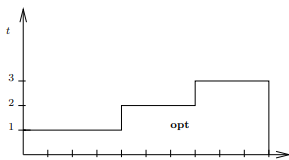
\includegraphics[]{chapters/introduction/histogram_opt.png}
        
        Now we construct another histogram for the greedy solution. We have $m$ columns, one for every set $S_i$. We order the columns (i.e sets) in the order they are covered by the greedy algorithm but the height of each column, rather than the timestep at which it was covered is now the price, as defined previously. The total area of the histogram is exactly equal to $\textbf{price}=\textbf{greedy}$. \\
        
        What we want to show is that $\textbf{price}$ is at most 4 times $\textbf{opt}$. The way we show that is by shrinking the second histogram by a factor of 4 and show that it fits completely inside the optimal histogram. The way we do that is by shrinking the height and the width by a factor of 2. Therefore, for each column we have a height of $p_i / 2$ and the width of the histogram is now $m/2$. \\
        
        Now, we align the greedy histogram to the right of the optimal histogram so that it occupies the space from $m/2 + 1$ up to $m$ on the horizontal axis. Now we claim that the shrunk greedy histogram is completely inside the optimal histogram and therefore this proves Lemma \ref{l:static_greedy}.
        
        \begin{figure}
            \centering
            \begin{subfigure}{.5\textwidth}
              \centering
              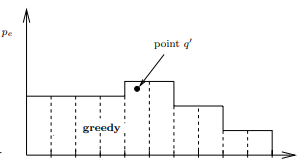
\includegraphics[width=.4\linewidth]{chapters/introduction/histogram_greedy.png}
              \caption{The greedy histogram before shrinking}
              \label{fig:sub1}
            \end{subfigure}%
            \begin{subfigure}{.5\textwidth}
              \centering
              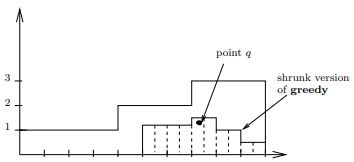
\includegraphics[width=.4\linewidth]{chapters/introduction/histogram_fit.png}
              \caption{Shrinking and Alignment}
              \label{fig:sub2}
            \end{subfigure}
            \label{fig:test}
        \end{figure}
        
        Consider an arbitrary point q' in the original (unshrunk) greedy histogram and let $S$ be the set it corresponds to. Let $i$ be the time step at which it was covered, then the height of this column is at most $\frac{|R_i|}{|X_i|}$ and the distance of q' from the right boundary of the optimal histogram is at most $R_i$. Now by shrinking we map the point q' to a new point q. The height of this point is now $h \leq \frac{|R_i|}{2 \cdot |X_i|}$ and the its distance from the right boundary is at most $r \leq \frac{|R_i|}{2}$. \\
        
        For our point q to lie within the optimal histogram it suffices to show that at timestep h at least r sets remain uncovered by the optimal algorithm. Consider the sets on $R_i$. No number can ever cover more than $|X_i|$ sets since our greedy algorithm selects at every time step the number that covers the most sets (and that is $|X_i$ at time step $i$). Therefore in $\floor{h}$ steps the optimal algorithm could cover at most $\floor{h} \cdot \floor{|X_i|} \leq \frac{|R_i|}{2}$ sets and therefore leave at least $|R_i| - \frac{|R_i|}{2} \geq \ceil{r}$ sets uncovered which proves our proposition that q lies within the optimal histogram.
    \end{proof}
    
    By the proof of Lemma \ref{l:static_greedy} we obtain that $\textbf{opt} \geq \textbf{price} / 4$ and since $\textbf{price} = \textbf{greedy}$ we have the proof of our original lemma.
    
\end{proof}

A natural question is whether the approximation ratio of this algorithm can be improved. To answer that we present the following hardness result.

\begin{theorem}\label{t:mssc_hardness}
    For every $\epsilon > 0$ it is NP-Hard to approximate min sum set cover within a ratio of $4-\epsilon$.
\end{theorem}

The authors of \cite{FLT04} continue by proving equivalent results for constrained versions of the problem as well as for the Min-Sum Vertex Cover, in which essentially every set $S_i$ has a cardinality of 2. Even though the algorithms they propose build an interesting intuition regarding the problem as we move on to generalized versions of the problem we observe that purely combinatorial tools are not sufficient to tackle the problem. This observation leads to the use of Linear Programming Relaxation methods which we use extensively while deriving our own results. To get a better idea of an Linear Programming approach we study a natural Generalization of the Min-Sum Set Cover problem \cite{SW11} and a randomized rounding schema that highlights several techniques. 

\section{The Generalized Min-Sum Set Cover}

After presenting the static version of Min Sum Set Cover we proceed with the generalization of the problem which was first introduced by Azar, Gamzu and Yin in \cite{AGY09}. In this problem we are once again given a universe $U$ with $|U| = n$, a collection of subsets of $U$, $S_1, S_2, ..., S_m \subseteq U$ and also an integer number for each set in the collection $K(S_i)$. Our purpose is to compute a permutation of $U$ in order to minimize the covering cost of each set: $\sum_{i=1}^{m} C( S_i )$ where $C(S_i)$ is the position of the $K(S_i)$-th element of $S_i$ that appears on the permutation. \\

In \cite{AGY09} the authors present an $O(logr)$-approximation algorithm where $r = max_{i} \{ |S_i| \}$. Subsequently, a constant factor approximation algorithm was given \cite{BGK10} based on Linear Programming. \\

In this section we present the main results of \cite{SW11} where the authors use a method called $\alpha$-point scheduling which helps them round the Linear Programming Relaxation of the problem and they obtain an algorithm that has a significantly better approximation ratio than \cite{BGK10}. The following results and techniques are rather important since several ideas we used for extracting our own results for $\DSSC$ are based on \cite{SW11}. \\

The first step is solving the following Linear Programming Relaxation of the problem. We define the variables $y_{i,t}$ which we want to be 1 if and only if $C(S_i) < t$ (that is, the $K(S_i)$-th element of the set $S_i$ appears before index t) and additionally the variables $x_{e,t}$ which we want to equal 1 if and only if the element e $e \in U$ appears at position $t$. Of course these hold for the integer program and since we solve a relaxation these variables will probably not be exactly equal to 1. Based on the constraints above we have the following linear program.

\begin{equation*}
    \begin{array}{ll@{}ll}
        \text min & \displaystyle \sum_{t = 1}^n \sum_{i = 1}^{m} ( 1 - y_{i,t} ) &\\
        \text{ s.t } & \displaystyle \sum_{e \in U} x_{e,t} = 1~~~~\text{για κάθε }t \leq n &&\\
        & \displaystyle \sum_{t=1}^{n} x_{e,t} = 1~~~~\text{για κάθε }e \in U &&\\
        & \displaystyle \sum_{e \in S \setminus A} \sum_{t'<t} x_{e,t} \geq (K(S_i) - |A|) \cdot y_{i,t}~~~~\text{ για κάθε } i \leq m, A \subseteq S_i, t \leq n &&\\
        & \displaystyle x_{e,t}, y_{i,t} \in [ 0, 1 ] ~~~~\text{ για κάθε } e \in U, i \leq m, t \leq n
    \end{array}
\end{equation*}

The Linear Program at first glance seems to have exponentially many constraints, since we create a constraint for every subset of every set $S_i$. It was shown in \cite{BGK10} that this problem can be dealt with and the exponentially many constraints can be separated in polynomial time so that we can solve the LP efficiently. \\

The basic algorithm for solving the problem with 28 appriximation ratio is based on $\alpha$ point scheduling. Specifically, for every $e \in U$ we select independently and uniformly $\alpha_e \in [0,1]$. Let $t_{e,\alpha_e}$ be the first time $t'$ s.t $\sum_{t=1}^{t'} x_{e,t} \geq \alpha_e$. We form the final permutation by ordering the elements $e \in U$ in decreasing order of $t_{e,\alpha_e}$ by breaking ties arbitrarily (but consistently). For more details on the analysis of the algorithm the interested reader may refer to \cite{BGK10}.

\section{The Online Version of Min Sum Set Cover}

\noindent
Before we formally introduce $\DSSC$ we present the results for the Online Version of Multistage Min-Sum Set Cover \cite{FKKSV20}. In this version we are given the request sets $S_t$ one by one without knowing in advance what requests may come in the future. At each timestep $t$, the set $S_t$ is revealed and we need to select a permutation $\pi^t$ to serve this request. To move from permutation $\pi^{t-1}$ to $\pi^t$ our algorithm pays $d_{KT} (\pi^{t-1}, \pi^t)$ where $d_{KT}$ denotes the Kendall-Tau distance. Our goal is to minimize $\sum_{t=1}^T \pi^t(S_t) + d_{KT} (\pi^{t-1}, \pi^t)$. \\

In \cite{FKKSV20} the authors investigate the Online Version of Min-Sum Set Cover. They notice that even though Online Min-Sum Set Cover is a generalization of List Update (List Update is a special case of Online Min-Sum Set Cover where all the request sets have cardinality 1, $|S_t| = 1$) the Move-to-Front which is the standard algorithm that achieves the optimal competitive ratio for List Update does not give any interesting results. In the future, as we proceed we consider that the request sets are $r$-uniform, that is $|S_t| = r \text{ for all } t \in [T]$.

\subsection{A Memoryless Algorithm for Online Min-Sum Set Cover}

The first result we present from the corresponding paper is a memoryless algorithm for Online Min-Sum Set Cover. An online algorithm is called memoryless iff the choices at timestep $t$ are not dependent on previous timesteps. We present the Move-All-Equally(MAE) Algorithm. Essentially what we do is that when we receive a request set $S_t$ we move every element of $S_t$ in the current permutation $\pi^{t-1}$ to the left until one of them reaches the head of the permutation. The algorithm is outlined below.

\begin{algorithm}[ht]
  \caption{Move-All-Equally}\label{alg:MAE}
  \textbf{Input:} The given request at time t $S_t$ and the permutation $\pi^{t-1}$.\\
  \textbf{Output:} A permutation at time $t$ $\pi^t$.

 \begin{algorithmic}[1]
    \STATE $k_t \leftarrow min\{ i | \pi^{t-1} [ i ] \in S_t \}$
    \STATE decrease the index of all elements on $S_t$ by $k_t - 1$.

  \end{algorithmic}
\end{algorithm}

This algorithm is quite interesting since it has 2 very interesting properties.

\begin{itemize}
    \item Let $e_t$ denote the element used by the optimal offline algorithm to cover the request $S_t$. Algorithm \ref{alg:MAE} moves this element towards the front of the list.
    \item It balances movement and access costs. If the access cost of the request $S_t$ is $k_t$ the movement cost of the algorithm is roughly $r \cdot k_t$. The basic idea is that the moving cost of algorithm \ref{alg:MAE} can be compensated by the decrease in the position of element $e_t$. This is why it is crucial all the elements to be moved with the same speed.
\end{itemize} 

Even though Algorithm \ref{alg:MAE} possesses these two interesting properties the authors show that it doesn't quite bridge the lower bound with a matching competitive ratio.

\begin{lemma}
    The Competitive Ratio of Algorithm \ref{alg:MAE} is $\Omega( r^2 )$.
\end{lemma}

\begin{proof}
    To construct an adversarial input sequence for our lower bound we request every time the last $r$ elements of the current permutation. Since Algorithm $\ref{alg:MAE}$ moves all the elements at the same speed we construct $n/r$ requests that are mutually disjoint. Therefore, we can serve each request optimally with a cost of $\Theta(n/r)$ whereas our MAE algorithm serves each request with a cost of $\Omega(n \cdot r)$. Therefore by comparing we obtain the lower bound on the competitive ratio.
\end{proof}

Even though the analysis of this algorithm doesn't allow for a matching upper bound the authors provide us with the following result. For more details on the analysis of the algorithm the interested reader may refer to \cite{FKKSV20}.

\begin{lemma}
    The Competitive Ratio of Algorithm \ref{alg:MAE} is at most $O( 2^{\sqrt( logn \cdot logr ) } ).$
\end{lemma}

\subsection{The Lazy Rounding Algorithm}

In this section we present a lower bound for every deterministic algorithm for Online Min-Sum Set Cover and further on we present the Lazy Rounding algorithm which is a deterministic algorithm that matches the lower bound (up to constant factors).

\begin{theorem}
    Any deterministic algorithm for the Online Min-Sum Set Cover problem has a competitive ratio at least $(r+1)(1 - \frac{1}{n+1})$.
\end{theorem}

For proving this Theorem the authors use an averaging argument, similar to that of List-Update \cite{ST85}. In each step the adversary requests once again the last $r$ elements of the current permutation and therefore the access cost is at least (n-r+1). By using simple counting techniques they show that for any fixed set $S_t$ of size $r$ and any $i \in [n-r+1]$, the number of permutations $\pi$ with access cost $\pi(S_t)=i$ is $\binom{n-i}{r-1} \cdot r! \cdot (n-r)!$. By summing over all permutations and dividing by $n!$ to get the average cost we get that the optimal permutation has cost at least $\frac{n+1}{r+1}$ and the competitive ratio of any algorithm is at lteat $(r+1)(1 - \frac{1}{n+1})$. For more details the interested reader may refer to the original paper. \\

Before stating the Lazy Rounding Algorithm and the main results we mention some of the algorithms that may sound natural but behave trivially bad. What's interesting is that this behaviour translates directly even in the offline version of the problem so it's interesting to know what absolutely doesn't work and motivate a non-combinatorial approach for the $\DSSC$.

\begin{itemize}
    \item \textbf{$MTF_{first}$}: Move to the front of the permutation the element of $S_t$ that appears first in $\pi^t$.
    \item \textbf{$MTF_{last}$}: Move to the front of the permutation the element of $S_t$ that appears last in $\pi^t$.
    \item \textbf{$MTF_{random}$}: Move a random element of $S_t$ to the front of the list.
\end{itemize}

All these algorithms have a tight $O(n)$ competitive ratio. Below we highlight the main parts of the Lazy Rounding algorithm which has an $O(r)$ competitive ratio. \\

\begin{enumerate}
    \item Use a black-box Multiplicative Weights Update Algorithm (MWU) with learning rate $1/n^3$. Using the results from learning theory the authors show that: $AccessCost(MWU) \leq \frac{5}{4} AccessCost(OPT)$.
    
    \item Using an online rounding scheme which turns any randomized algorithm A to a deterministic one, denoted $Derand(A)$, with access cost at most $2r \cdot \mathbb{R}[AccessCost(A)]$, without any guarantee so far for the Moving Cost of $Derand(A)$.
    
    \item Lazy-Rounding is essentially a lazy version of $Derand(MWU)$ (applying the online rounding scheme to the Multiplicative Weights Update Algorithm) that updates the permutation only if the distribution of MWU has changed a lot. Let's call a time interval where Lazy-Rounding does not change it's permutation a phase. The authors show that during a phase:
        \begin{itemize}
            \item $AccessCost(Lazy-Rounding) \leq 4r \cdot \mathbb{E}[AccessCost(MWU)]$.
            \item $MovingCost(Lazy-Rounding) \leq \mathbb{E}[AccessCost(MWU)]$.
        \end{itemize}
\end{enumerate}

By combining the above properties we obtain: $$Cost(Lazy-Rounding) \leq (4r+1) \mathbb{E}[AccessCost(MWU)] \leq (5r+2) Cost(OPT)$$.

\begin{theorem}
    The deterministic online algorithm Lazy-Rounding is (5r+2) competitive for the Online Version of Min-Sum Set Cover.
\end{theorem}

\section{The Multistage Min-Sum Set Cover}

\subsection{Problem Definition}
\label{s:intro}

In \emph{Multistage Min-Sum Set Cover} ($\DSSC$), we are given a universe $U$ on $n$ elements, a sequence of requests $\cR = (R_1, \ldots, R_T)$, with $R_t \subseteq U$, and an initial permutation $\pi^0$ of the elements of $U$. We aim to maintain a sequence of permutations $(\pi^0, \pi^1, \ldots, \pi^T)$ of $U$, so as to minimize the total cost of updating (or moving from) $\pi^{t-1}$ to $\pi^{t}$ in each time step plus the total cost of covering each request $R_t$ with the current permutation $\pi^t$. The cost of moving from $\pi^{t-1}$ to $\pi^{t}$ is the number of inverted element pairs between $\pi^{t-1}$ and $\pi^t$, i.e., the Kendall Tau distance $\dkt(\pi^{t-1}, \pi^t)$. The cost $\pi^t(R_t)$ of covering a request $R_t$ with a permutation $\pi^t$ is the position of the first element of $R_t$ in $\pi^t$, i.e., $\pi^t(R_t) = \min\{ i \,|\, \pi^t(i) \in R_t \}$. Thus, given $\cR = (R_1, \ldots, R_T)$, we aim to minimize $\sum_{t=1}^T \big( \dkt(\pi^{t-1}, \pi^t) + \pi^t(R_t) \big)$. 
%
%More formally, given $U$ and $\cR = \{ R_1, \ldots, R_T \}$, the goal in $\DSSC$ is to maintain a sequence of permutations $\pi^0, \pi^1, \ldots, \pi^T$ so as to minimize the total moving cost plus the total covering cost: $\sum_{t=1}^T \big( \dkt(\pi^{t-1}, \pi^t) + \pi^t(R_t) \big)$. 

The $\DSSC$ problem is a natural generalization of the (offline version of the) classical \emph{List Update} problem \cite{ST85b}, where $|R_t| = 1$ for all requests $R_t \in \cR$. The offline version of List Update is $\mathrm{NP}$-hard \cite{Amb00}, while it is known that any $5/4$-approximation has to resort to \emph{paid exchanges}, where an element different from the requested one is moved forward to the list \cite{LRR15,tim16}. $\DSSC$ was introduced in \cite{FKKSV20} as the multistage extension of Min-Sum Set Cover ($\SSC$) \cite{FLT04}, where we aim to compute a single static permutation $\pi$ that minimizes the total covering cost  $\sum_{t=1}^T \pi(R_t)$. \cite{FKKSV20} presented a (simple polynomial-time) online algorithm for $\DSSC$ with competitive ratio between $\Omega(r \sqrt{n})$ and $O(r^{3/2} \sqrt{n})$ for $r$-bounded instances, where all requests have cardinality at most $r$, and posed the polynomial-time approximability of $\DSSC$ as an interesting open question. $\DSSC$ is also related to recently studied time-evolving (a.k.a. multistage or dynamic) optimization problems (e.g., multistage matroid, spanning set and perfect matching maintenance \cite{GTW14}, time-evolving Facility Location \cite{EMS14,Svensson15}), where we aim to maintain a sequence of near-optimal feasible solutions to a combinatorial optimization problem, in response to time-evolving underlying costs, without changing too much the solution from one step to the next. 
%We elaborate on the connections of $\DSSC$ to previous work in Section~\ref{s:related}. 

\subsection{Motivation}

%
$\DSSC$ is motivated by applications, such as web search, news, online shopping, paper bidding, etc., where items are presented to the users sequentially. Then, the item ranking is of paramount importance, because user attention is usually restricted to the first few items in the sequence (see e.g., \cite{StreeterGK09,CKMS01,FSR18,PT18}). If a user does not spot an item fitting her interests there, she either leaves the service (in case of news or online shopping, see e.g., the empirical evidence in \cite{DGMM20}) or settles on a suboptimal action (in case of paper bidding, see e.g., \cite{GP13}). To mitigate such situations and increase user retention, modern online services highly optimize item rankings based on user scrolling and click patterns. Each user $t$ is represented by her set of preferred items (or item categories) $R_t$\,. The goal of the service provider is to continually maintain an item ranking $\pi^t$, so that the current user $t$ finds one of her favorite items at a relatively high position in $\pi^t$. Continual ranking update is dictated by the fact that users with different characteristics and preferences tend to use the online service during the course of the day (e.g., elderly people in the morning, middle-aged people in the evening, young people at the night -- similar patterns apply for people from different countries and timezones). Moreover, different user categories react in nonuniform ways to different trends (in e.g., news, fashion, sports, scientific topics). For consistency and stability, however, the ranking should change neither too much nor too frequently. $\DSSC$ makes the (somewhat simplifying) assumptions that the service provider has a relatively accurate knowledge of user preferences and their arrival order, and that its total cost is proportional to how deep in $\pi^t$ the current user $t$ should reach, before she finds one of her favorite items, and to how much the ranking changes from one user to the next. 

From a theoretical viewpoint, $\DSSC$ was used in \cite{FKKSV20} as a natural benchmark for studying the dynamic competitive ratio of Online Min-Sum Set Cover, where the algorithm updates its permutation online, without any knowledge of future requests. As in $\DSSC$, the objective is to minimize the total moving plus the total covering cost. 

\subsection{Our Contribution and Techniques.}
%
In this work, we initiate a study of the polynomial-time approximability of $\DSSC$. Using a reduction from Set Cover, we show (Theorem~\ref{t:hardness}) that $\DSSC$ does not admit a $c\log n$-approximation, for some absolute constant $c$, unless $\mathrm{P}=\mathrm{NP}$. Moreover our reduction establishes that an $o(r)$-approximation for $r$-bounded instances of $\DSSC$ implies an $o(r)$-approximation for Set Cover, in case each element appears in at most $r$ requests. 

Our main technical contribution is to show that $\DSSC$ can be approximated in polynomial-time within a factor of $O(\log^2 n)$ in general instances, by randomized rounding (Theorem~\ref{t:rand}), and within a factor of $O(r^2)$ in $r$-bounded instances, by deterministic rounding (Theorem~\ref{t:greedy}). %Both results require a novel approach and several key new insights related to the dynamic nature of $\DSSC$. 

For both results, we consider a restricted version of $\DSSC$, inspired by the Move-to-Front (MTF) algorithm for List Update, where in each time step $t$, we can only move a single element of $R_t$ from its position in $\pi^{t-1}$ to the first position of $\pi^t$. Since such a permutation $\pi^t$ coves $R_t$ with unit cost, we now aim to select the element of each $R_t$ moved to front of $\pi^t$, so as to minimize the total moving cost $\sum_{t=1}^T \dkt(\pi^{t-1}, \pi^t)$. It is not hard to see that the optimal cost of serving $\cR$ under the restricted Move-to-Front version of $\DSSC$ is within a factor of $4$ from the optimal cost under the original, more general, definition of $\DSSC$. 

Hence, approximating $\DSSC$ boils down to determining which element of $R_t$ should become the top element of $\pi^{t}$. To this end, we relax permutations to doubly stochastic matrices and consider a Linear Programming relaxation of the restricted Move-to-Front version of $\DSSC$, which we call \emph{Fractional-MTF} (see Definition~\ref{d:frac_MTF}). Given the optimal solution of the aforementioned linear program, which is a sequence of doubly stochastic matrices $(A^0, A^1, \ldots, A^T)$, with $A^0$ corresponding to the initial permutation $\pi^0$, our main technical challenge is to round each doubly stochastic matrix $A^t$ to a permutation $\pi^t$ such that (i) there is an element of $R_t$ at one of the few top positions of $\pi^t$; and (ii) the total moving cost $\sum_{t=1}^T \dkt(\pi^{t-1}, \pi^t)$ of the rounded solution is comparable to the total moving cost $\sum_{t=1}^T \dfr(A^{t-1}, A^t)$ of the optimal solution of Fractional-MTF, where $\dfr$ is a notion of distance equivalent to Spearman's footrule distance on permutations (see Definition~\ref{d:distance_lp}).

Working towards a randomized rounding approach, we first observe that rounding each doubly stochastic matrix independently may result in a permutation sequence with total moving cost significantly larger than that of Fractional-MTF (see also the discussion after Lemma~\ref{l:relax}). In Theorem~\ref{t:rand}, we show that a dependent randomized rounding with  logarithmic scaling of entries  (Algorithm~\ref{alg:rand_rounding}), similar in spirit with the randomized rounding approach \cite{BGK10,SW11} for Generalized Min-Sum Set Cover, results in an approximation ratio of $O(\log^2 n)$. Interestingly, Algorithm~\ref{alg:rand_rounding} without the logarithmic scaling results in a permutation sequence with the expected moving cost within a factor of $4$ from the optimal moving cost of Fractional-MTF. However, we lose a logarithmic factor in the approximation ratio, because we need to scale up the entries of each doubly stochastic matrix $A^t$, so as to ensure that some element of $R_t$ appears in the few top positions of $\pi^t$ with sufficiently large probability. The other logarithmic factor is lost because there could be a logarithmic number of elements allocated to the same position of the resulting permutation by the randomized rounding. 

Our deterministic rounding of Algorithm~\ref{alg:greedy_rounding} for $r$-bounded request sequences is motivated by the deterministic rounding for Set Cover and Vertex Cover. We observe that in the optimal solution of Fractional-MTF, in each time step $t$, there is some element $e \in R_t$ with $A^{t}_{e1} \geq 1/r$ (i.e., $e$ occupies a fraction of at least $1/r$ of the first position in the ``fractional permutation'' $A^t$). Algorithm~\ref{alg:greedy_rounding} simply moves any such element to the front of $\pi^t$. The most challenging part of the analysis is to establish that for any optimal solution $(A^0, A^1, \ldots, A^T)$ of Fractional-MTF with respect to an $r$-bounded request sequence, there exists a sequence of doubly stochastic matrices $(A^0, \hat{A}^1, \ldots, \hat{A}^T)$ with the entries of each $\hat{A}^t$ being multiples of $1/r$, such that (i) the moving cost of $(A^0, \hat{A}^1, \ldots, \hat{A}^T)$ is bounded from above by the optimal cost of Fractional-MTF; and (ii) each matrix $\hat{A}^t$ contains in the first position the element that Algorithm~\ref{alg:greedy_rounding} keeps in the first position at round $t$, with mass at least $1/r$. Then we show (Lemma~\ref{l:r_integral}) that for any sequence of doubly stochastic matrices $(A^0, \hat{A}^1, \ldots, \hat{A}^T)$ satisfying the above properties, the moving cost of Algorithm~\ref{alg:greedy_rounding} is at most the moving cost of the doubly stochastic matrices,
$\sum_{t=1}^T \dfr(\hat{A}^t,\hat{A}^{t-1})$. The latter is done through the use of an appropriate potential function based on an extension of the Kendall-Tau distance to doubly stochastic matrix with entries being multiples of $1/r$.

A potentially interesting insight %from the analysis of our rounding schemes 
is that the technical reason for the quadratic dependence of our approximation ratios on $\log n$ and $r$ is conceptually similar to the reason for the (best possible) approximation ratio of $4 = 2\cdot 2$ in \cite{FLT04} (see the discussion after Theorem~\ref{t:rand}). Hence, we conjecture that any $o(\log^2 n)$ (resp. $o(r^2)$) approximation to $\DSSC$ must imply a sublogarithmic (resp. $o(r)$) approximation to Set Cover.% (resp. where each element appears at most $r$ times). 

%In addition to making significant progress towards understanding the polynomial-time approximability of $\DSSC$, we believe that the techniques applied to the analysis of our rounding schemes may be of independent interest and may find applications to the design of approximation algorithms for other time-evolving and/or dynamic optimization problems. 